% ==============================================================================
% ================================= Aufgabe 6 =================================
% ==============================================================================

\chapter{Aufgabe 6: Auswertung der Umfragedaten}
\label{chap:aufgabe6}
\thispagestyle{fancy}

In dieser Aufgabe wird die Datei \texttt{report.php} implementiert, die eine einfache Auswertung der Umfragedaten anzeigt.

\section{Logik der \texttt{report.php}}

Die Datei \texttt{report.php} führt drei \acs{SQL}-Abfragen aus und zeigt die Ergebnisse in einer Liste an:

\begin{enumerate}
    \item Anzahl der angemeldeten Personen (\textit{nicht anonym})
    \item Anzahl der anonymen Teilnahmen
    \item Gesamtzahl der Teilnahmen
\end{enumerate}

\subsection{Vollständiger Quellcode}

\lstinputlisting[
    language=php,
    caption={Auswertung der Umfragedaten in \texttt{report.php}},
    label={lst:report-php}
]{asset/code/Aufgabe6.tex}

\subsection{Erläuterung der \acs{SQL}-Abfragen}

\subsubsection{Angemeldete Personen}

Die Anzahl der angemeldeten Personen wird mit folgender Abfrage ermittelt:

\begin{lstlisting}[language=sql]
SELECT COUNT(DISTINCT s.UserId) AS count
FROM survey_table s
JOIN user_table u ON s.UserId = u.Id
WHERE u.Name != 'anonymous'
\end{lstlisting}

Dabei wird \texttt{DISTINCT} verwendet, um jeden Nutzer nur einmal zu zählen, auch wenn er mehrfach an der Umfrage teilgenommen hat.

\subsubsection{Anonyme Personen}

Die Anzahl der anonymen Teilnahmen wird mit folgender Abfrage ermittelt:

\begin{lstlisting}[language=sql]
SELECT COUNT(*) AS count
FROM survey_table s
JOIN user_table u ON s.UserId = u.Id
WHERE u.Name = 'anonymous'
\end{lstlisting}

Hier wird jeder Eintrag gezählt, da ein Nutzer mehrfach anonym teilnehmen kann.

\subsubsection{Gesamt}

Die Gesamtzahl der Teilnahmen wird mit folgender Abfrage ermittelt:

\begin{lstlisting}[language=sql]
SELECT COUNT(*) FROM survey_table
\end{lstlisting}

\subsection{Ausgabe}

Die Ausgabe erfolgt als einfache Liste mit den drei Werten:

\begin{figure}[h]
    \centering
    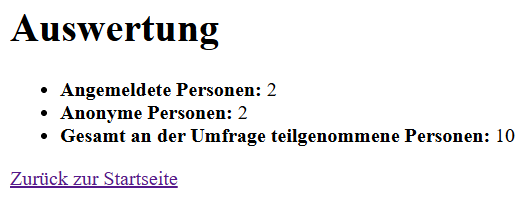
\includegraphics[width=0.7\textwidth]{./asset/image/Aufgabe6.png}
    \caption[Auswertung der Umfragedaten (\textit{Quelle: Eigene Darstellung})]
            {Auswertung der Umfragedaten (\textit{Quelle: Eigene Darstellung})\\ 
            \url{http://localhost/survey/report.php}}
    \label{fig:report}
\end{figure}

\section{Zusammenfassung}

Die Auswertung der Umfragedaten wurde erfolgreich implementiert:

\begin{itemize}
    \item Die Anzahl der angemeldeten Personen wird korrekt ermittelt.
    \item Die Anzahl der anonymen Teilnahmen wird korrekt ermittelt.
    \item Die Gesamtzahl der Teilnahmen wird korrekt ermittelt.
    \item Die Ausgabe erfolgt übersichtlich in einer Liste.
\end{itemize}

Die Datei \texttt{report.php} liegt unter folgendem Pfad:

\begin{forest}
    for tree={
        font=\ttfamily,
        grow'=0,
        child anchor=west,
        parent anchor=south,
        anchor=west,
        calign=first,
        edge path={
            \noexpand\path [draw, \forestoption{edge}] (!u.south west) +(10pt,0) |- node[fill,inner sep=1.5pt] {} (.child anchor)\forestoption{edge label};
        },
        before typesetting nodes={
            if n=1{
                insert before={[,phantom,calign with current]}
            }{}
        },
        fit=band,
        before computing xy={l=22pt},
    }
    [\textbf{C:\textbackslash xampp\textbackslash htdocs\textbackslash survey}
        [\textbf{report.php}]
    ]
\end{forest}

Die Anwendung ist nun vollständig implementiert und alle Aufgaben sind abgeschlossen.

% ==============================================================================
% =================================== Aufgabe 6 ================================
% ==============================================================================